% Options for packages loaded elsewhere
\PassOptionsToPackage{unicode}{hyperref}
\PassOptionsToPackage{hyphens}{url}
%
\documentclass[
]{article}
\usepackage{amsmath,amssymb}
\usepackage{lmodern}
\usepackage{iftex}
\ifPDFTeX
  \usepackage[T1]{fontenc}
  \usepackage[utf8]{inputenc}
  \usepackage{textcomp} % provide euro and other symbols
\else % if luatex or xetex
  \usepackage{unicode-math}
  \defaultfontfeatures{Scale=MatchLowercase}
  \defaultfontfeatures[\rmfamily]{Ligatures=TeX,Scale=1}
\fi
% Use upquote if available, for straight quotes in verbatim environments
\IfFileExists{upquote.sty}{\usepackage{upquote}}{}
\IfFileExists{microtype.sty}{% use microtype if available
  \usepackage[]{microtype}
  \UseMicrotypeSet[protrusion]{basicmath} % disable protrusion for tt fonts
}{}
\makeatletter
\@ifundefined{KOMAClassName}{% if non-KOMA class
  \IfFileExists{parskip.sty}{%
    \usepackage{parskip}
  }{% else
    \setlength{\parindent}{0pt}
    \setlength{\parskip}{6pt plus 2pt minus 1pt}}
}{% if KOMA class
  \KOMAoptions{parskip=half}}
\makeatother
\usepackage{xcolor}
\usepackage[margin=1in]{geometry}
\usepackage{color}
\usepackage{fancyvrb}
\newcommand{\VerbBar}{|}
\newcommand{\VERB}{\Verb[commandchars=\\\{\}]}
\DefineVerbatimEnvironment{Highlighting}{Verbatim}{commandchars=\\\{\}}
% Add ',fontsize=\small' for more characters per line
\usepackage{framed}
\definecolor{shadecolor}{RGB}{248,248,248}
\newenvironment{Shaded}{\begin{snugshade}}{\end{snugshade}}
\newcommand{\AlertTok}[1]{\textcolor[rgb]{0.94,0.16,0.16}{#1}}
\newcommand{\AnnotationTok}[1]{\textcolor[rgb]{0.56,0.35,0.01}{\textbf{\textit{#1}}}}
\newcommand{\AttributeTok}[1]{\textcolor[rgb]{0.77,0.63,0.00}{#1}}
\newcommand{\BaseNTok}[1]{\textcolor[rgb]{0.00,0.00,0.81}{#1}}
\newcommand{\BuiltInTok}[1]{#1}
\newcommand{\CharTok}[1]{\textcolor[rgb]{0.31,0.60,0.02}{#1}}
\newcommand{\CommentTok}[1]{\textcolor[rgb]{0.56,0.35,0.01}{\textit{#1}}}
\newcommand{\CommentVarTok}[1]{\textcolor[rgb]{0.56,0.35,0.01}{\textbf{\textit{#1}}}}
\newcommand{\ConstantTok}[1]{\textcolor[rgb]{0.00,0.00,0.00}{#1}}
\newcommand{\ControlFlowTok}[1]{\textcolor[rgb]{0.13,0.29,0.53}{\textbf{#1}}}
\newcommand{\DataTypeTok}[1]{\textcolor[rgb]{0.13,0.29,0.53}{#1}}
\newcommand{\DecValTok}[1]{\textcolor[rgb]{0.00,0.00,0.81}{#1}}
\newcommand{\DocumentationTok}[1]{\textcolor[rgb]{0.56,0.35,0.01}{\textbf{\textit{#1}}}}
\newcommand{\ErrorTok}[1]{\textcolor[rgb]{0.64,0.00,0.00}{\textbf{#1}}}
\newcommand{\ExtensionTok}[1]{#1}
\newcommand{\FloatTok}[1]{\textcolor[rgb]{0.00,0.00,0.81}{#1}}
\newcommand{\FunctionTok}[1]{\textcolor[rgb]{0.00,0.00,0.00}{#1}}
\newcommand{\ImportTok}[1]{#1}
\newcommand{\InformationTok}[1]{\textcolor[rgb]{0.56,0.35,0.01}{\textbf{\textit{#1}}}}
\newcommand{\KeywordTok}[1]{\textcolor[rgb]{0.13,0.29,0.53}{\textbf{#1}}}
\newcommand{\NormalTok}[1]{#1}
\newcommand{\OperatorTok}[1]{\textcolor[rgb]{0.81,0.36,0.00}{\textbf{#1}}}
\newcommand{\OtherTok}[1]{\textcolor[rgb]{0.56,0.35,0.01}{#1}}
\newcommand{\PreprocessorTok}[1]{\textcolor[rgb]{0.56,0.35,0.01}{\textit{#1}}}
\newcommand{\RegionMarkerTok}[1]{#1}
\newcommand{\SpecialCharTok}[1]{\textcolor[rgb]{0.00,0.00,0.00}{#1}}
\newcommand{\SpecialStringTok}[1]{\textcolor[rgb]{0.31,0.60,0.02}{#1}}
\newcommand{\StringTok}[1]{\textcolor[rgb]{0.31,0.60,0.02}{#1}}
\newcommand{\VariableTok}[1]{\textcolor[rgb]{0.00,0.00,0.00}{#1}}
\newcommand{\VerbatimStringTok}[1]{\textcolor[rgb]{0.31,0.60,0.02}{#1}}
\newcommand{\WarningTok}[1]{\textcolor[rgb]{0.56,0.35,0.01}{\textbf{\textit{#1}}}}
\usepackage{graphicx}
\makeatletter
\def\maxwidth{\ifdim\Gin@nat@width>\linewidth\linewidth\else\Gin@nat@width\fi}
\def\maxheight{\ifdim\Gin@nat@height>\textheight\textheight\else\Gin@nat@height\fi}
\makeatother
% Scale images if necessary, so that they will not overflow the page
% margins by default, and it is still possible to overwrite the defaults
% using explicit options in \includegraphics[width, height, ...]{}
\setkeys{Gin}{width=\maxwidth,height=\maxheight,keepaspectratio}
% Set default figure placement to htbp
\makeatletter
\def\fps@figure{htbp}
\makeatother
\setlength{\emergencystretch}{3em} % prevent overfull lines
\providecommand{\tightlist}{%
  \setlength{\itemsep}{0pt}\setlength{\parskip}{0pt}}
\setcounter{secnumdepth}{-\maxdimen} % remove section numbering
\ifLuaTeX
  \usepackage{selnolig}  % disable illegal ligatures
\fi
\IfFileExists{bookmark.sty}{\usepackage{bookmark}}{\usepackage{hyperref}}
\IfFileExists{xurl.sty}{\usepackage{xurl}}{} % add URL line breaks if available
\urlstyle{same} % disable monospaced font for URLs
\hypersetup{
  pdftitle={Solutions for assignment 7},
  pdfauthor={Guy Roberts},
  hidelinks,
  pdfcreator={LaTeX via pandoc}}

\title{Solutions for assignment 7}
\author{Guy Roberts}
\date{2023-03-04}

\begin{document}
\maketitle

\hypertarget{solution-to-1.1}{%
\subsection{Solution to 1.1}\label{solution-to-1.1}}

In order to answer this question, we used trial and error of varying
values of \(\alpha\), this is because we know that:

\begin{align*}
    Pr(N \leq 2) &= \pi(2) + \pi(1) + \pi(0)
\end{align*}

We find that our solution is approximately \(\alpha \approx 0.4349\)
from using our function defined earlier.

\begin{align*}
  \int_{1}^{\infty}\beta^{-2}d\beta &= \biggl[ -\beta^{-1} \biggr]_{1}^{\infty} = 0 + 1 = 1
\end{align*}

Hence, our prior is a probability density function.

\hypertarget{solution-to-1.2}{%
\subsection{Solution to 1.2}\label{solution-to-1.2}}

The mode for an Inverse-Gamma distribution with parameters \(\alpha\)
and \(\beta\) is defined as \(\frac{\beta}{\alpha+1}\). So for
\(\sigma^{2}\) the prior mode will be \(\frac{1}{11}\).

And for the prior mode of \(\beta\), we do not have a prior mode, since
the function is undefined at \(\beta = 0\).

\hypertarget{solution-to-1.3}{%
\subsection{Solution to 1.3}\label{solution-to-1.3}}

\begin{Shaded}
\begin{Highlighting}[]
\NormalTok{data \{}
\NormalTok{  int\textless{}lower=0\textgreater{} N; // num obs}
\NormalTok{  vector[N] x;    // obs explanatory}
\NormalTok{  vector[N] y;    // obs response}
\NormalTok{\}}

\NormalTok{parameters \{}
\NormalTok{  real beta;           // gradient}
\NormalTok{  real\textless{}lower=0\textgreater{} sigma; // error std.}
\NormalTok{\}}

\NormalTok{model \{}
\NormalTok{  // Priors}
\NormalTok{  target += {-}2 * log(beta); // prior for beta}
\NormalTok{  target += inv\_gamma\_lpdf(sigma | 0.1, 0.1); // prior on sigma\^{}2}
  
\NormalTok{  // Likelihood}
\NormalTok{  target += normal\_lpdf(y | beta * x, sigma);}
\NormalTok{\}}
\end{Highlighting}
\end{Shaded}

\hypertarget{solution-to-1.4}{%
\subsection{Solution to 1.4}\label{solution-to-1.4}}

\begin{Shaded}
\begin{Highlighting}[]
\FunctionTok{library}\NormalTok{(rstan)}

\NormalTok{our\_data }\OtherTok{=} \FunctionTok{list}\NormalTok{(}
  \AttributeTok{N =} \DecValTok{8}\NormalTok{,}
  \AttributeTok{x =} \FunctionTok{c}\NormalTok{(}\FloatTok{2.13}\NormalTok{, }\FloatTok{4.32}\NormalTok{, }\FloatTok{3.60}\NormalTok{, }\FloatTok{0.19}\NormalTok{, }\FloatTok{5.62}\NormalTok{, }\FloatTok{2.86}\NormalTok{, }\FloatTok{4.50}\NormalTok{, }\FloatTok{1.95}\NormalTok{),}
  \AttributeTok{y =} \FunctionTok{c}\NormalTok{(}\FloatTok{4.02}\NormalTok{, }\FloatTok{8.73}\NormalTok{, }\FloatTok{7.33}\NormalTok{, }\FloatTok{0.51}\NormalTok{, }\FloatTok{12.09}\NormalTok{, }\FloatTok{5.99}\NormalTok{, }\FloatTok{8.91}\NormalTok{, }\FloatTok{4.02}\NormalTok{)}
\NormalTok{)}

\FunctionTok{setwd}\NormalTok{(}\StringTok{\textquotesingle{}C:/Users/guyro/Desktop/DU/Maths/Y3/bayesian{-}modelling/assignments/assignment7\textquotesingle{}}\NormalTok{)}

\NormalTok{model }\OtherTok{=} \FunctionTok{stan\_model}\NormalTok{(}\StringTok{\textquotesingle{}model1.stan\textquotesingle{}}\NormalTok{)}
\NormalTok{fit }\OtherTok{=} \FunctionTok{sampling}\NormalTok{(model, our\_data, }\AttributeTok{chains=}\DecValTok{4}\NormalTok{, }\AttributeTok{iter=}\DecValTok{10000}\NormalTok{, }\AttributeTok{warmup=}\DecValTok{500}\NormalTok{, }\AttributeTok{thin=}\DecValTok{1}\NormalTok{)}
\end{Highlighting}
\end{Shaded}

\begin{verbatim}
## 
## SAMPLING FOR MODEL 'anon_model' NOW (CHAIN 1).
## Chain 1: 
## Chain 1: Gradient evaluation took 4.1e-05 seconds
## Chain 1: 1000 transitions using 10 leapfrog steps per transition would take 0.41 seconds.
## Chain 1: Adjust your expectations accordingly!
## Chain 1: 
## Chain 1: 
## Chain 1: Iteration:    1 / 10000 [  0%]  (Warmup)
## Chain 1: Iteration:  501 / 10000 [  5%]  (Sampling)
## Chain 1: Iteration: 1500 / 10000 [ 15%]  (Sampling)
## Chain 1: Iteration: 2500 / 10000 [ 25%]  (Sampling)
## Chain 1: Iteration: 3500 / 10000 [ 35%]  (Sampling)
## Chain 1: Iteration: 4500 / 10000 [ 45%]  (Sampling)
## Chain 1: Iteration: 5500 / 10000 [ 55%]  (Sampling)
## Chain 1: Iteration: 6500 / 10000 [ 65%]  (Sampling)
## Chain 1: Iteration: 7500 / 10000 [ 75%]  (Sampling)
## Chain 1: Iteration: 8500 / 10000 [ 85%]  (Sampling)
## Chain 1: Iteration: 9500 / 10000 [ 95%]  (Sampling)
## Chain 1: Iteration: 10000 / 10000 [100%]  (Sampling)
## Chain 1: 
## Chain 1:  Elapsed Time: 0.017 seconds (Warm-up)
## Chain 1:                0.25 seconds (Sampling)
## Chain 1:                0.267 seconds (Total)
## Chain 1: 
## 
## SAMPLING FOR MODEL 'anon_model' NOW (CHAIN 2).
## Chain 2: Rejecting initial value:
## Chain 2:   Log probability evaluates to log(0), i.e. negative infinity.
## Chain 2:   Stan can't start sampling from this initial value.
## Chain 2: Rejecting initial value:
## Chain 2:   Log probability evaluates to log(0), i.e. negative infinity.
## Chain 2:   Stan can't start sampling from this initial value.
## Chain 2: Rejecting initial value:
## Chain 2:   Log probability evaluates to log(0), i.e. negative infinity.
## Chain 2:   Stan can't start sampling from this initial value.
## Chain 2: Rejecting initial value:
## Chain 2:   Log probability evaluates to log(0), i.e. negative infinity.
## Chain 2:   Stan can't start sampling from this initial value.
## Chain 2: Rejecting initial value:
## Chain 2:   Log probability evaluates to log(0), i.e. negative infinity.
## Chain 2:   Stan can't start sampling from this initial value.
## Chain 2: 
## Chain 2: Gradient evaluation took 6e-06 seconds
## Chain 2: 1000 transitions using 10 leapfrog steps per transition would take 0.06 seconds.
## Chain 2: Adjust your expectations accordingly!
## Chain 2: 
## Chain 2: 
## Chain 2: Iteration:    1 / 10000 [  0%]  (Warmup)
## Chain 2: Iteration:  501 / 10000 [  5%]  (Sampling)
## Chain 2: Iteration: 1500 / 10000 [ 15%]  (Sampling)
## Chain 2: Iteration: 2500 / 10000 [ 25%]  (Sampling)
## Chain 2: Iteration: 3500 / 10000 [ 35%]  (Sampling)
## Chain 2: Iteration: 4500 / 10000 [ 45%]  (Sampling)
## Chain 2: Iteration: 5500 / 10000 [ 55%]  (Sampling)
## Chain 2: Iteration: 6500 / 10000 [ 65%]  (Sampling)
## Chain 2: Iteration: 7500 / 10000 [ 75%]  (Sampling)
## Chain 2: Iteration: 8500 / 10000 [ 85%]  (Sampling)
## Chain 2: Iteration: 9500 / 10000 [ 95%]  (Sampling)
## Chain 2: Iteration: 10000 / 10000 [100%]  (Sampling)
## Chain 2: 
## Chain 2:  Elapsed Time: 0.011 seconds (Warm-up)
## Chain 2:                0.153 seconds (Sampling)
## Chain 2:                0.164 seconds (Total)
## Chain 2: 
## 
## SAMPLING FOR MODEL 'anon_model' NOW (CHAIN 3).
## Chain 3: 
## Chain 3: Gradient evaluation took 8e-06 seconds
## Chain 3: 1000 transitions using 10 leapfrog steps per transition would take 0.08 seconds.
## Chain 3: Adjust your expectations accordingly!
## Chain 3: 
## Chain 3: 
## Chain 3: Iteration:    1 / 10000 [  0%]  (Warmup)
## Chain 3: Iteration:  501 / 10000 [  5%]  (Sampling)
## Chain 3: Iteration: 1500 / 10000 [ 15%]  (Sampling)
## Chain 3: Iteration: 2500 / 10000 [ 25%]  (Sampling)
## Chain 3: Iteration: 3500 / 10000 [ 35%]  (Sampling)
## Chain 3: Iteration: 4500 / 10000 [ 45%]  (Sampling)
## Chain 3: Iteration: 5500 / 10000 [ 55%]  (Sampling)
## Chain 3: Iteration: 6500 / 10000 [ 65%]  (Sampling)
## Chain 3: Iteration: 7500 / 10000 [ 75%]  (Sampling)
## Chain 3: Iteration: 8500 / 10000 [ 85%]  (Sampling)
## Chain 3: Iteration: 9500 / 10000 [ 95%]  (Sampling)
## Chain 3: Iteration: 10000 / 10000 [100%]  (Sampling)
## Chain 3: 
## Chain 3:  Elapsed Time: 0.014 seconds (Warm-up)
## Chain 3:                0.11 seconds (Sampling)
## Chain 3:                0.124 seconds (Total)
## Chain 3: 
## 
## SAMPLING FOR MODEL 'anon_model' NOW (CHAIN 4).
## Chain 4: Rejecting initial value:
## Chain 4:   Log probability evaluates to log(0), i.e. negative infinity.
## Chain 4:   Stan can't start sampling from this initial value.
## Chain 4: Rejecting initial value:
## Chain 4:   Log probability evaluates to log(0), i.e. negative infinity.
## Chain 4:   Stan can't start sampling from this initial value.
## Chain 4: Rejecting initial value:
## Chain 4:   Log probability evaluates to log(0), i.e. negative infinity.
## Chain 4:   Stan can't start sampling from this initial value.
## Chain 4: Rejecting initial value:
## Chain 4:   Log probability evaluates to log(0), i.e. negative infinity.
## Chain 4:   Stan can't start sampling from this initial value.
## Chain 4: Rejecting initial value:
## Chain 4:   Log probability evaluates to log(0), i.e. negative infinity.
## Chain 4:   Stan can't start sampling from this initial value.
## Chain 4: Rejecting initial value:
## Chain 4:   Log probability evaluates to log(0), i.e. negative infinity.
## Chain 4:   Stan can't start sampling from this initial value.
## Chain 4: Rejecting initial value:
## Chain 4:   Log probability evaluates to log(0), i.e. negative infinity.
## Chain 4:   Stan can't start sampling from this initial value.
## Chain 4: 
## Chain 4: Gradient evaluation took 7e-06 seconds
## Chain 4: 1000 transitions using 10 leapfrog steps per transition would take 0.07 seconds.
## Chain 4: Adjust your expectations accordingly!
## Chain 4: 
## Chain 4: 
## Chain 4: Iteration:    1 / 10000 [  0%]  (Warmup)
## Chain 4: Iteration:  501 / 10000 [  5%]  (Sampling)
## Chain 4: Iteration: 1500 / 10000 [ 15%]  (Sampling)
## Chain 4: Iteration: 2500 / 10000 [ 25%]  (Sampling)
## Chain 4: Iteration: 3500 / 10000 [ 35%]  (Sampling)
## Chain 4: Iteration: 4500 / 10000 [ 45%]  (Sampling)
## Chain 4: Iteration: 5500 / 10000 [ 55%]  (Sampling)
## Chain 4: Iteration: 6500 / 10000 [ 65%]  (Sampling)
## Chain 4: Iteration: 7500 / 10000 [ 75%]  (Sampling)
## Chain 4: Iteration: 8500 / 10000 [ 85%]  (Sampling)
## Chain 4: Iteration: 9500 / 10000 [ 95%]  (Sampling)
## Chain 4: Iteration: 10000 / 10000 [100%]  (Sampling)
## Chain 4: 
## Chain 4:  Elapsed Time: 0.012 seconds (Warm-up)
## Chain 4:                0.145 seconds (Sampling)
## Chain 4:                0.157 seconds (Total)
## Chain 4:
\end{verbatim}

\begin{verbatim}
## Warning: There were 8597 divergent transitions after warmup. See
## https://mc-stan.org/misc/warnings.html#divergent-transitions-after-warmup
## to find out why this is a problem and how to eliminate them.
\end{verbatim}

\begin{verbatim}
## Warning: Examine the pairs() plot to diagnose sampling problems
\end{verbatim}

\begin{verbatim}
## Warning: The largest R-hat is 1.55, indicating chains have not mixed.
## Running the chains for more iterations may help. See
## https://mc-stan.org/misc/warnings.html#r-hat
\end{verbatim}

\begin{verbatim}
## Warning: Bulk Effective Samples Size (ESS) is too low, indicating posterior means and medians may be unreliable.
## Running the chains for more iterations may help. See
## https://mc-stan.org/misc/warnings.html#bulk-ess
\end{verbatim}

\begin{verbatim}
## Warning: Tail Effective Samples Size (ESS) is too low, indicating posterior variances and tail quantiles may be unreliable.
## Running the chains for more iterations may help. See
## https://mc-stan.org/misc/warnings.html#tail-ess
\end{verbatim}

\begin{Shaded}
\begin{Highlighting}[]
\FunctionTok{print}\NormalTok{(fit, }\AttributeTok{pars=}\FunctionTok{c}\NormalTok{(}\StringTok{"beta"}\NormalTok{, }\StringTok{"sigma"}\NormalTok{))}
\end{Highlighting}
\end{Shaded}

\begin{verbatim}
## Inference for Stan model: anon_model.
## 4 chains, each with iter=10000; warmup=500; thin=1; 
## post-warmup draws per chain=9500, total post-warmup draws=38000.
## 
##       mean se_mean   sd 2.5%  25%  50%  75% 97.5% n_eff  Rhat
## beta  1.54    0.63 0.89  0.0 1.34 2.04 2.07  2.12     2 31.04
## sigma 1.47    1.39 1.97  0.2 0.28 0.35 2.68  4.87     2 21.88
## 
## Samples were drawn using NUTS(diag_e) at Wed Mar  8 20:02:44 2023.
## For each parameter, n_eff is a crude measure of effective sample size,
## and Rhat is the potential scale reduction factor on split chains (at 
## convergence, Rhat=1).
\end{verbatim}

\begin{Shaded}
\begin{Highlighting}[]
\CommentTok{\# Extract the posterior samples for beta and sigma}
\NormalTok{beta\_samples }\OtherTok{=} \FunctionTok{extract}\NormalTok{(fit)}\SpecialCharTok{$}\NormalTok{beta}
\NormalTok{sigma\_samples }\OtherTok{=} \FunctionTok{extract}\NormalTok{(fit)}\SpecialCharTok{$}\NormalTok{sigma}
\NormalTok{sigma2\_samples }\OtherTok{=}\NormalTok{ sigma\_samples}\SpecialCharTok{\^{}}\DecValTok{2}

\FunctionTok{hist}\NormalTok{(beta\_samples)}
\end{Highlighting}
\end{Shaded}

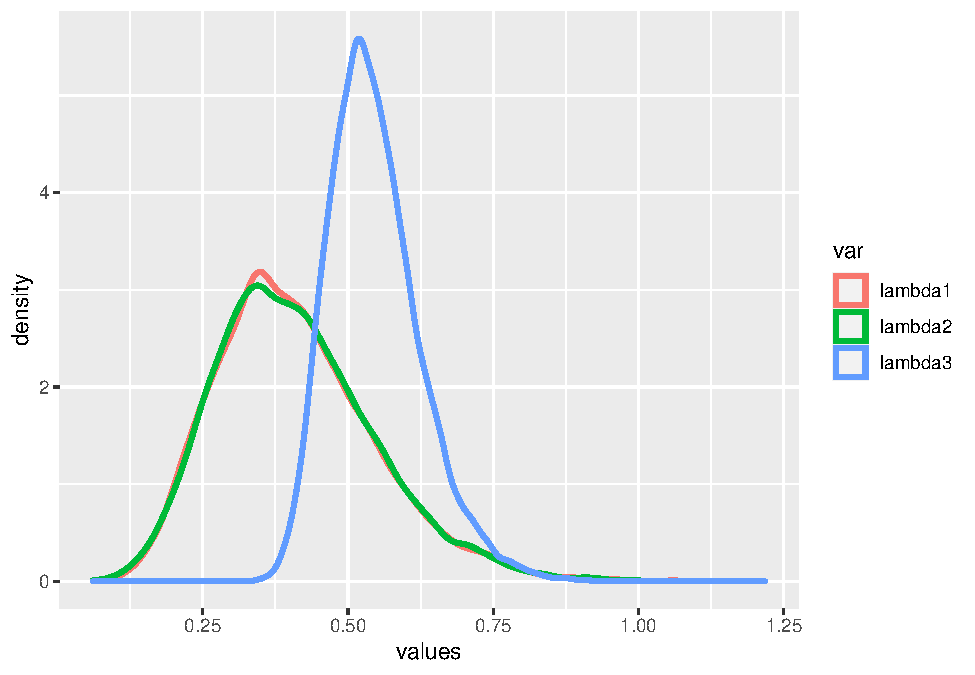
\includegraphics{Assignment-7_files/figure-latex/unnamed-chunk-1-1.pdf}

\begin{Shaded}
\begin{Highlighting}[]
\FunctionTok{hist}\NormalTok{(sigma2\_samples)}
\end{Highlighting}
\end{Shaded}

\includegraphics{Assignment-7_files/figure-latex/unnamed-chunk-1-2.pdf}

\hypertarget{solution-to-2.1}{%
\subsection{Solution to 2.1}\label{solution-to-2.1}}

\begin{Shaded}
\begin{Highlighting}[]
\NormalTok{data \{}
\NormalTok{  int\textless{}lower=0\textgreater{} N;}
\NormalTok{  int\textless{}lower=0\textgreater{} x[N];}
\NormalTok{\}}

\NormalTok{parameters \{}
\NormalTok{  real\textless{}lower=0\textgreater{} lambda;}
\NormalTok{\}}

\NormalTok{model \{}
\NormalTok{  // Prior}
\NormalTok{  lambda \textasciitilde{} frechet(2, 4);}
  
\NormalTok{  // Likelihood (Comment out to sample from preposterior)}
\NormalTok{  //for (i in 1:N) \{}
\NormalTok{  //  x[i] \textasciitilde{} poisson(lambda[i]);}
\NormalTok{  //\}}
\NormalTok{\}}
\end{Highlighting}
\end{Shaded}

\hypertarget{solution-to-2.2}{%
\subsection{Solution to 2.2}\label{solution-to-2.2}}

\begin{Shaded}
\begin{Highlighting}[]
\FunctionTok{library}\NormalTok{(rstan)}
\NormalTok{N }\OtherTok{=} \DecValTok{3} \CommentTok{\# no. data points}
\NormalTok{x }\OtherTok{=} \FunctionTok{c}\NormalTok{(}\DecValTok{1}\NormalTok{, }\DecValTok{3}\NormalTok{, }\DecValTok{2}\NormalTok{) }\CommentTok{\# some random count data}
\NormalTok{our\_data }\OtherTok{=} \FunctionTok{list}\NormalTok{(}\AttributeTok{N =}\NormalTok{ N, }\AttributeTok{x =}\NormalTok{ x)}

\NormalTok{model2 }\OtherTok{=} \FunctionTok{stan\_model}\NormalTok{(}\StringTok{\textquotesingle{}model2.stan\textquotesingle{}}\NormalTok{)}
\NormalTok{fit }\OtherTok{=} \FunctionTok{sampling}\NormalTok{(model2, our\_data, }\AttributeTok{iter=}\DecValTok{10000}\NormalTok{)}
\end{Highlighting}
\end{Shaded}

\begin{verbatim}
## 
## SAMPLING FOR MODEL 'anon_model' NOW (CHAIN 1).
## Chain 1: 
## Chain 1: Gradient evaluation took 2.4e-05 seconds
## Chain 1: 1000 transitions using 10 leapfrog steps per transition would take 0.24 seconds.
## Chain 1: Adjust your expectations accordingly!
## Chain 1: 
## Chain 1: 
## Chain 1: Iteration:    1 / 10000 [  0%]  (Warmup)
## Chain 1: Iteration: 1000 / 10000 [ 10%]  (Warmup)
## Chain 1: Iteration: 2000 / 10000 [ 20%]  (Warmup)
## Chain 1: Iteration: 3000 / 10000 [ 30%]  (Warmup)
## Chain 1: Iteration: 4000 / 10000 [ 40%]  (Warmup)
## Chain 1: Iteration: 5000 / 10000 [ 50%]  (Warmup)
## Chain 1: Iteration: 5001 / 10000 [ 50%]  (Sampling)
## Chain 1: Iteration: 6000 / 10000 [ 60%]  (Sampling)
## Chain 1: Iteration: 7000 / 10000 [ 70%]  (Sampling)
## Chain 1: Iteration: 8000 / 10000 [ 80%]  (Sampling)
## Chain 1: Iteration: 9000 / 10000 [ 90%]  (Sampling)
## Chain 1: Iteration: 10000 / 10000 [100%]  (Sampling)
## Chain 1: 
## Chain 1:  Elapsed Time: 0.057 seconds (Warm-up)
## Chain 1:                0.059 seconds (Sampling)
## Chain 1:                0.116 seconds (Total)
## Chain 1: 
## 
## SAMPLING FOR MODEL 'anon_model' NOW (CHAIN 2).
## Chain 2: 
## Chain 2: Gradient evaluation took 3e-06 seconds
## Chain 2: 1000 transitions using 10 leapfrog steps per transition would take 0.03 seconds.
## Chain 2: Adjust your expectations accordingly!
## Chain 2: 
## Chain 2: 
## Chain 2: Iteration:    1 / 10000 [  0%]  (Warmup)
## Chain 2: Iteration: 1000 / 10000 [ 10%]  (Warmup)
## Chain 2: Iteration: 2000 / 10000 [ 20%]  (Warmup)
## Chain 2: Iteration: 3000 / 10000 [ 30%]  (Warmup)
## Chain 2: Iteration: 4000 / 10000 [ 40%]  (Warmup)
## Chain 2: Iteration: 5000 / 10000 [ 50%]  (Warmup)
## Chain 2: Iteration: 5001 / 10000 [ 50%]  (Sampling)
## Chain 2: Iteration: 6000 / 10000 [ 60%]  (Sampling)
## Chain 2: Iteration: 7000 / 10000 [ 70%]  (Sampling)
## Chain 2: Iteration: 8000 / 10000 [ 80%]  (Sampling)
## Chain 2: Iteration: 9000 / 10000 [ 90%]  (Sampling)
## Chain 2: Iteration: 10000 / 10000 [100%]  (Sampling)
## Chain 2: 
## Chain 2:  Elapsed Time: 0.053 seconds (Warm-up)
## Chain 2:                0.053 seconds (Sampling)
## Chain 2:                0.106 seconds (Total)
## Chain 2: 
## 
## SAMPLING FOR MODEL 'anon_model' NOW (CHAIN 3).
## Chain 3: 
## Chain 3: Gradient evaluation took 4e-06 seconds
## Chain 3: 1000 transitions using 10 leapfrog steps per transition would take 0.04 seconds.
## Chain 3: Adjust your expectations accordingly!
## Chain 3: 
## Chain 3: 
## Chain 3: Iteration:    1 / 10000 [  0%]  (Warmup)
## Chain 3: Iteration: 1000 / 10000 [ 10%]  (Warmup)
## Chain 3: Iteration: 2000 / 10000 [ 20%]  (Warmup)
## Chain 3: Iteration: 3000 / 10000 [ 30%]  (Warmup)
## Chain 3: Iteration: 4000 / 10000 [ 40%]  (Warmup)
## Chain 3: Iteration: 5000 / 10000 [ 50%]  (Warmup)
## Chain 3: Iteration: 5001 / 10000 [ 50%]  (Sampling)
## Chain 3: Iteration: 6000 / 10000 [ 60%]  (Sampling)
## Chain 3: Iteration: 7000 / 10000 [ 70%]  (Sampling)
## Chain 3: Iteration: 8000 / 10000 [ 80%]  (Sampling)
## Chain 3: Iteration: 9000 / 10000 [ 90%]  (Sampling)
## Chain 3: Iteration: 10000 / 10000 [100%]  (Sampling)
## Chain 3: 
## Chain 3:  Elapsed Time: 0.053 seconds (Warm-up)
## Chain 3:                0.054 seconds (Sampling)
## Chain 3:                0.107 seconds (Total)
## Chain 3: 
## 
## SAMPLING FOR MODEL 'anon_model' NOW (CHAIN 4).
## Chain 4: 
## Chain 4: Gradient evaluation took 3e-06 seconds
## Chain 4: 1000 transitions using 10 leapfrog steps per transition would take 0.03 seconds.
## Chain 4: Adjust your expectations accordingly!
## Chain 4: 
## Chain 4: 
## Chain 4: Iteration:    1 / 10000 [  0%]  (Warmup)
## Chain 4: Iteration: 1000 / 10000 [ 10%]  (Warmup)
## Chain 4: Iteration: 2000 / 10000 [ 20%]  (Warmup)
## Chain 4: Iteration: 3000 / 10000 [ 30%]  (Warmup)
## Chain 4: Iteration: 4000 / 10000 [ 40%]  (Warmup)
## Chain 4: Iteration: 5000 / 10000 [ 50%]  (Warmup)
## Chain 4: Iteration: 5001 / 10000 [ 50%]  (Sampling)
## Chain 4: Iteration: 6000 / 10000 [ 60%]  (Sampling)
## Chain 4: Iteration: 7000 / 10000 [ 70%]  (Sampling)
## Chain 4: Iteration: 8000 / 10000 [ 80%]  (Sampling)
## Chain 4: Iteration: 9000 / 10000 [ 90%]  (Sampling)
## Chain 4: Iteration: 10000 / 10000 [100%]  (Sampling)
## Chain 4: 
## Chain 4:  Elapsed Time: 0.053 seconds (Warm-up)
## Chain 4:                0.061 seconds (Sampling)
## Chain 4:                0.114 seconds (Total)
## Chain 4:
\end{verbatim}

\begin{Shaded}
\begin{Highlighting}[]
\NormalTok{samples }\OtherTok{=} \FunctionTok{extract}\NormalTok{(fit, }\AttributeTok{pars=}\FunctionTok{c}\NormalTok{(}\StringTok{\textquotesingle{}x\_prepost[1]\textquotesingle{}}\NormalTok{, }\StringTok{\textquotesingle{}x\_prepost[2]\textquotesingle{}}\NormalTok{, }\StringTok{\textquotesingle{}x\_prepost[3]\textquotesingle{}}\NormalTok{))}
\FunctionTok{plot}\NormalTok{(}\FunctionTok{density}\NormalTok{(samples}\SpecialCharTok{$}\StringTok{\textasciigrave{}}\AttributeTok{x\_prepost[1]}\StringTok{\textasciigrave{}}\NormalTok{))}
\end{Highlighting}
\end{Shaded}

\includegraphics{Assignment-7_files/figure-latex/unnamed-chunk-2-1.pdf}

\hypertarget{solution-to-2.3}{%
\subsection{Solution to 2.3}\label{solution-to-2.3}}

One solution would be to add some constraints to the model. From the
lectures in Chapter 10, we could truncate our model, in order to force
the generated samples to be greater than 4. Essentially adding a lower
bound. However, this would mean that no samples would be less than 4,
which isn't exactly what we want.

Alternatively, we could modify our prior distribution for \(lambda\) to
``shift'' the density further from 4. For example, we use the location
parameter, \(m\) of the Frechet distribution. Though I am not entirely
sure how to implement this in Stan, since the distribution only takes in
the scale and shape parameters, not the location parameter, \(m\).

\end{document}
